\documentclass[t]{beamer}

% Load general definitions
% Preamble file - general definitions, package loading, etc.

%=================================
% Load packages
\usepackage{amssymb,amsmath}
\usepackage{graphicx}
\usepackage{url}
\usepackage{tikz}
\usetikzlibrary{mindmap,trees,arrows}
\usepackage{fancyvrb}
\usepackage[english]{babel}
\usepackage[latin1]{inputenc}
\usepackage{subfigure}
\usepackage{times}
\usepackage[T1]{fontenc}
\usepackage{cancel}
\usepackage{color}
\usepackage{listings}

%=================================
% Set mode
\mode<presentation>
{
	\usetheme{Madrid}
	\usecolortheme{whale}
	\useoutertheme{infolines}
	\setbeamercovered{invisible}
}

% Get rid of nav bar
\beamertemplatenavigationsymbolsempty

% Insert frame number at bottom of the page.
\usefoottemplate{\hfil\tiny{\color{black!90}\insertframenumber}} 

%=================================
% Define new commands

\newcommand\Real{{\mathbb{R}}}
%\newcommand{\vi}{\vspace{0.6\baselineskip}}
%\newcommand{\goodgap}{\hspace{\subfigtopskip}\hspace{\subfigbottomskip}}


% Equation environments
\newcommand{\beq}{\begin{equation}}
\newcommand{\eq}{\end{equation}}
\newcommand{\beqs}{\begin{equation*}}
\newcommand{\eqs}{\end{equation*}}
\newcommand{\beqn}{\begin{eqnarray}}
\newcommand{\eqn}{\end{eqnarray}}

% Bold variables
\newcommand{\mbf}[1]{\ensuremath{\mathbf{#1}}}

% Itemization
\newcommand{\bitem}{\begin{itemize}}
\newcommand{\eitem}{\end{itemize}}
\newcommand{\spitem}{\vskip 1em\item}
\newcommand{\bitems}{\begin{itemize}\item}
\newcommand{\benums}{\begin{enumerate}\item}
\newcommand{\eenum}{\end{enumerate}}

% color blocks
\newenvironment{colorblock}[2]{%
\setbeamercolor{block title}{#2}
\begin{block}{#1}}{\end{block}}

% Vertical spacing
\newcommand{\vone}{\vskip 1em}
\newcommand{\vhalf}{\vskip .5em}

% Frame environments
\newenvironment{ftst}[3][t]{%
\begin{frame}{environment=ftst,#1}
\frametitle{#2}
\framesubtitle{#3}}{\end{frame}}

\newenvironment{ftstf}[2]{
\begin{frame}[fragile,environment=ftstf]
\frametitle{#1}
\framesubtitle{#2}}{\end{frame}}

% colors
\definecolor{MyGray}{rgb}{0.5,0.5,0.5}
\definecolor{MyDBGray}{rgb}{0.1,0.1,0.4}
\definecolor{darkgreen}{rgb}{0,0.4,0}
\definecolor{black}{rgb}{0,0,0}
\def\defn#1{{\color{red} #1}}

% Footnote
\renewcommand{\thefootnote}{\alph{footnote}}

% Relaxed footnotes
\newcommand{\lfr}[1]{\let\thefootnote\relax\footnote{\tiny #1}}

% Verbatim environment - using FANCYVRB package
\DefineVerbatimEnvironment%
{rcode}{Verbatim}
{fontsize=\scriptsize}

% Verbatim environment - using LISTINGS package
%\lstnewenvironment{rcode} {\lstset{	language = R,
%									basicstyle = \scriptsize\ttfamily,
%									showspaces = false,
%									showstringspaces = false,
%									showtabs = false,
%									keywordstyle = \color{black}\bfseries,
%									commentstyle = \color{darkgreen},
%									numbers = none,
%									otherkeywords={	<-,
%													ggplot,
%													geom_boxplot,
%													facet_grid,
%													shapiro.test,
%													fligner.test,
%													glht,
%													with},
%									deletekeywords={data,
%													model,
%													residuals,
%													c,
%													axis,
%													default,
%													labels,
%													qq.text}}}%
%{}


% Specific definitions
\title[]{Design and Analysis of Experiments}
\subtitle[]{09 - Non-normal data}
\author[]{Felipe Campelo\\{\footnotesize http://orcslab.cpdee.ufmg.br/}}
\institute{Graduate Program in Electrical Engineering}
\date{\scriptsize Belo Horizonte\\April 2015}

\begin{document}

% cover page
\setbeamertemplate{footline}{}
\begin{frame}
\begin{flushright}

\includegraphics[width=.25\textwidth]{../figs/principal_completa3_ufmg}
\end{flushright}
  \titlepage
  \begin{tikzpicture}[remember picture,overlay]
  \node[anchor=south east,xshift=-5pt,yshift=122pt] at (current page.south east) {\tiny Version 2.11};
  \node[anchor=south west,yshift=0pt] at (current page.south west) {
\includegraphics[width=.15\textwidth]{../figs/by-nc-sa.png}};
  \end{tikzpicture}  
\end{frame}

%=====

% quotation page
  \begin{frame}[b]
		\frametitle{}
\begin{columns}[T]
\column{0.77\textwidth}
\flushright{\small ``\textit{Nothing has such power to broaden the mind\\
as the ability to investigate systematically and truly
\\all that comes under thy observation in life.}''\\\ \\
Marcus Aurelius Antoninus Augustus\\
121 -- 180\\
Roman emperor and stoic philosopher.\\}
\column{0.23\textwidth}
\begin{tikzpicture}[remember picture,overlay]
\node[anchor=south east,yshift=25pt,xshift=0pt] at (current page.south east)
{
\includegraphics[width=2\textwidth]{../figs/aurelius.png}};
\end{tikzpicture}
\end{columns}
\vhalf
\lfr{Image: \url{http://www.yourbest100.com/people/top-100-philosophers/}}
\end{frame}

%=====
% Main slides

\begin{ftst}
{Simple comparisons}
{Non-normal data}
Up to this point, we have been using methods that rely on strong distributional assumptions - particularly on the assumption of \textit{normality} - to perform inference on mean values;
\vone
The Central Limit Theorem allows this assumption to be relaxed in some cases (e.g., large sample sizes, unimodal symmetrical distributions, etc.); 
\vone
However, scientists and engineers frequently have to deal with data that does not conform with the normality assumption (relaxed or not) of traditional t-tests.
\begin{tikzpicture}[remember picture,overlay]
\node[anchor=south east,yshift=0pt,xshift=0pt] at (current page.south east)
{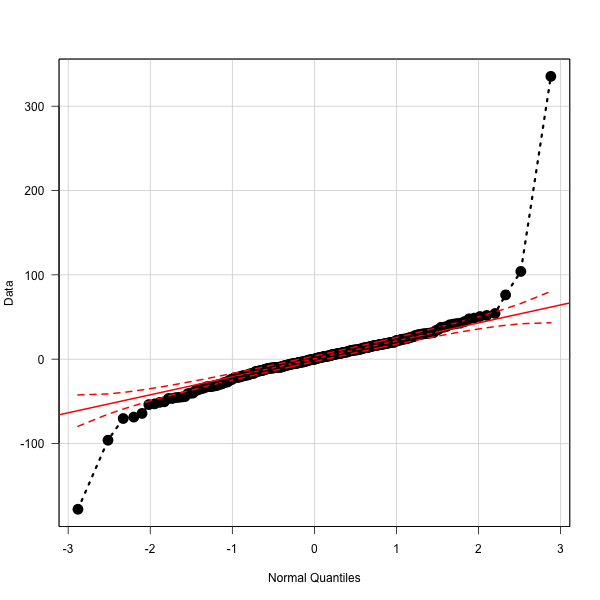
\includegraphics[width=.27\textwidth]{../figs/logn_qq.png}};
\node[anchor=south east,yshift=0pt,xshift=-100pt] at (current page.south east)
{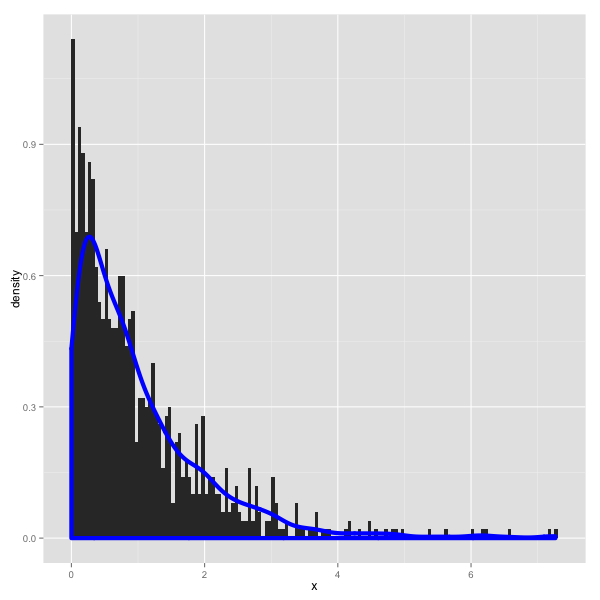
\includegraphics[width=.25\textwidth]{../figs/expdata.png}};
\end{tikzpicture}
\end{ftst}

%=====

\begin{ftst}
{Simple comparisons}
{Non-normal data}
The most common strategies to deal with non-normal samples are:

\bitems Data transformation;
\spitem Rank-based methods;
\spitem Bootstrap-based methods;
\spitem Distribution-specific methods.
\eitem
\vone
In this lecture we'll introduce the first three approaches. The use of distribution-specific methods (e.g., generalized linear models) will be discussed in future versions of this course.
\end{ftst}

%=====
% Part I: Data transformations
\begin{ftst}
{Data transformations}
{Main concepts}
It is very common for phenomena to present behaviors that can be characterized by distributions other than the normal;
\vone


\end{ftst}

%=====

\begin{ftst}
{Data transformations}
{Log transformation}

\end{ftst}

%=====

\begin{ftst}
{Data transformations}
{Square root transformation}

\end{ftst}

%=====

\begin{ftst}
{Data transformations}
{Other transformations}

\end{ftst}

%=====
% Part 2: Rank-based methods
\begin{ftst}
{Rank-based methods}
{Main concepts}

\end{ftst}

%=====

\begin{ftst}
{Rank-based methods}
{Inference on one median}

\end{ftst}

%=====

\begin{ftst}
{Rank-based methods}
{Inference on two medians}

\end{ftst}

%=====

\begin{ftst}
{Rank-based methods}
{Paired design}

\end{ftst}

%=====
% Part 3: Bootstrap methods
\begin{ftst}
{Bootstrap}
{Main concepts}

\end{ftst}

%=====

\begin{ftst}
{Bootstrap}
{Confidence intervals}

\end{ftst}

%=====

\begin{ftst}
{Bootstrap}
{Inference using bootstrap}

\end{ftst}

%=====

\begin{ftst}
{Final remarks}
{Some considerations}

\end{ftst}

%=====


\begin{ftst}
{Bibliography}
{\ }
\scriptsize
\textbf{Required reading}

\benums  %E. Walker, A.S. Nowacki, \textit{Understanding Equivalence and Noninferiority Testing}, Journal of General Internal Medicine 26(2):192-196, 2011.
\eenum

\textbf{Recommended reading}

\benums %P. Mathews, \textit{Sample Size Calculations: Practical Methods for Engineers and Scientists}, Ch. 2.4, 1st ed., MMB, 2010.
\item %P. Zhang, \textit{A Simple Formula for Sample Size Calculation in Equivalence Studies}, Journal of Biopharmaceutical Statistics 13(3):529-538, 2003.
\eenum
\end{ftst}

%=====

\begin{ftstf}{About this material}{Conditions of use and referencing}
\centering\footnotesize This work is licensed under the Creative Commons CC BY-NC-SA 4.0 license\\(Attribution Non-Commercial Share Alike International License version 4.0).\\
\vhalf
\url{http://creativecommons.org/licenses/by-nc-sa/4.0/}\\
\vone
\footnotesize Please reference this work as:\\
\footnotesize \flushleft Felipe Campelo (2015), \textit{Lecture Notes on Design and Analysis of Experiments}.\\Online: {\scriptsize\url{https://github.com/fcampelo/Design-and-Analysis-of-Experiments}}\\
Version 2.11, Chapter 9; Creative Commons BY-NC-SA 4.0.\\

\begin{Verbatim}[fontsize=\tiny]
    @Misc{Campelo2015-01,
      title={Lecture Notes on Design and Analysis of Experiments},
      author={Felipe Campelo},
      howPublished={\url{https://github.com/fcampelo/Design-and-Analysis-of-Experiments}},
      year={2015},
      note={Version 2.11, Chapter 9; Creative Commons BY-NC-SA 4.0.},
    }
\end{Verbatim}

\begin{tikzpicture} [remember picture,overlay]
\node[anchor=south,yshift=0pt] at (current page.south){ \includegraphics[width=.2\textwidth]{../figs/CCSomerights.png}};
\end{tikzpicture}
\end{ftstf}


\end{document}